%% Type de document et encodage de la police
\documentclass[a4paper]{article}
\usepackage[utf8x]{inputenc}
\usepackage[T1]{fontenc}
\usepackage[french]{babel}

%% Initialise la taille des pages et des marges
\usepackage[a4paper, top=3cm, bottom=3cm, left=2cm, right=2cm, marginparwidth=2cm]{geometry}

%% Packs utiles
\usepackage{amsmath}
\usepackage{graphicx}
\usepackage[colorinlistoftodos]{todonotes}
\usepackage{fourier-orns}
\usepackage{titlesec}
\usepackage{fancyhdr}
\usepackage{fancyvrb}
\usepackage{array}
\usepackage{enumitem}

%% Tabular Stuff
\renewcommand{\arraystretch}{1.2} % row 20 % longer
\usepackage{colortbl}
\newcommand{\bluecell}{\cellcolor{blue!25}}

%% colors
\definecolor{sprinen}{rgb}{0.0, 1.0, 0.7}

%% Packs utiles pour la manipulation d'image
\usepackage{wallpaper}
\usepackage{amsfonts}
\usepackage{amssymb}
\usepackage{eso-pic}
\usepackage{multicol}

%% \headrulewidth && \footrulewidth
\renewcommand{\headrulewidth}{1pt}
\fancyhead[R]{\footnotesize{\leftmark}}
\renewcommand{\footrulewidth}{1pt}
\fancyfoot[R]{\thepage}

%% Pour faire un encadré au coins arrondis
\usepackage{fancybox}
\cornersize{0.25}

%% Pour mettre une ligne à gauche d'une explication
\usepackage{mdframed}
\newmdenv[topline=false, bottomline=false, rightline=false, skipabove=\topsep, skipbelow=\topsep
]{example}

%% Pack Tikz pour les diagrammes
\usepackage{tikz}
\usetikzlibrary{shapes, shapes.geometric, arrows, decorations.pathmorphing, backgrounds, fit, petri, calc, patterns, decorations.pathreplacing, decorations.markings, tikzmark}

%% Noeuds -> diagrammes
\tikzstyle{rouge} = [
    rectangle,
    rounded corners,
    minimum width = 3cm,
    minimum height = 1cm,
    text centered,
    draw = black,
    fill = red!30
]
\tikzstyle{vert} = [
    diamond,
    minimum width = 3cm,
    minimum height = 1cm,
    text centered,
    draw = black,
    fill = green!30
]
\tikzstyle{incolore} = [
    rectangle,
    rounded corners,
    minimum width = 3cm,
    minimum height = 1cm,
    text centered,
    draw = black,
]

%% Formes -> ALU
\tikzstyle{ALU} = [ %% ATTENTION: pas de lignes vides dans "mark"
decoration = {
    markings,
    mark connection node = up-left,
    mark connection node = up-right,
    mark connection node = below,
    mark = at position 0 with {
        \coordinate (up-left) at (0,0);
        \coordinate (up-right) at (2.5,0);
        \coordinate (below) at (1.25,-2);
        \coordinate (center) at (1.25,-0.75);
        \draw[-] ($(up-left) + (-0.5,0)$) -- ($(up-left) + (0.5,0)$);
        \draw[-] ($(up-right) + (-0.5,0)$) -- ($(up-right) + (0.5,0)$);
        \draw[-] ($(below) + (-0.5,0)$) -- ($(below) + (0.5,0)$);
        \draw[-] ($(below) + (-0.5,0)$) -- ($(up-left) + (-0.5,0)$);
        \draw[-] ($(up-right) + (0.5,0)$) -- ($(below) + (0.5,0)$);
        \draw[-] ($(up-right) + (-0.5,0)$) -- (center);
        \draw[-] ($(up-left) + (0.5,0)$) -- (center);
        \node (text) at (1.25,-1.25) {\textbf{ALU}};
    }
}, decorate]



\title{Architecture des systèmes}
\author{Grégoire Roumache}
\date{Octobre 2019}

\begin{document}

\maketitle





\tableofcontents





\section{Concepts de base}





\subsection{Représentation n°1}

\begin{center}
%%  \textcolor{red}{\textbf{Instructions}} \textbf{+} \textcolor{blue}{\textbf{Données}} \textbf{=} \textcolor{magenta}{\textbf{Résultats}} \\

\begin{tikzpicture} [node distance = 1.5cm]
    \node (Instructions) [] {\textcolor{red}{\textbf{Instructions}}};
    \node (Données) [below of = Instructions] {\textcolor{blue}{\textbf{Données}}};

    \node (Ordinateur) [incolore, right of = Instructions, draw = black, yshift = -0.75cm, xshift = 2.5cm] {\textbf{Ordinateur}};

    \node (Résultats) [right of = Ordinateur, xshift = 2.5cm] {\textcolor{magenta}{\textbf{Résultats}}};

    \draw[-] (Instructions) -| ($(Ordinateur) - (2.5, 0)$);
    \draw[-] (Données) -| ($(Ordinateur) - (2.5, 0)$);
    \draw[->] ($(Ordinateur) - (2.5, 0)$) -- (Ordinateur);

    \draw[->] (Ordinateur) -- (Résultats);
\end{tikzpicture}
\end{center}

À retenir de ce modèle:
\begin{itemize}
    \item Les flux d'informations sont \textbf{continus}. (flux = instructions, données, résultats).
    \item L'ordinateur n'effectue que des opérations simples (ex: opérations arithmétiques).
\end{itemize}
\begin{example}
Exemple:
\begin{center}
\begin{tikzpicture} [node distance = 1.5cm]
    \node (Instructions) [] {\textcolor{red}{\textbf{Instruction: ADD}}};
    \node (Données) [below of = Instructions] {\textcolor{blue}{\textbf{Données: 1; 2}}};

    \node (Ordinateur) [incolore, right of = Instructions, draw = black, yshift = -0.75cm, xshift = 3cm] {\textbf{Ordinateur}};

    \node (Résultats) [right of = Ordinateur, xshift = 2.5cm] {\textcolor{magenta}{\textbf{Résultat: 3}}};

    \draw[-] (Instructions) -| ($(Ordinateur) - (2.5, 0)$);
    \draw[-] (Données) -| ($(Ordinateur) - (2.5, 0)$);
    \draw[->] ($(Ordinateur) - (2.5, 0)$) -- (Ordinateur);

    \draw[->] (Ordinateur) -- (Résultats);
\end{tikzpicture}
\end{center}
\end{example}





\subsection{Représentation n°2}

Représentation du processus:
\begin{center}
\begin{tikzpicture} [node distance = 1.5cm]
    \node (Instructions) [] {\textcolor{red}{\textbf{Instructions}}};
    \node (Données) [below of = Instructions] {\textcolor{blue}{\textbf{Données}}};

    \node (Ordinateur) [incolore, right of = Instructions, draw = black, yshift = -0.75cm, xshift = 2.5cm] {\textbf{Ordinateur}};

    \node (Résultats) [right of = Ordinateur, xshift = 2.5cm] {\textcolor{magenta}{\textbf{Résultats}}};

    \draw[-] (Instructions) -| ($(Ordinateur) - (2.5, 0)$);
    \draw[-] (Données) -| ($(Ordinateur) - (2.5, 0)$);
    \draw[->] ($(Ordinateur) - (2.5, 0)$) -- (Ordinateur);
    \draw[->] (Ordinateur) -- (Résultats);

    \coordinate (BelowRésultats) at ($(Résultats) + (0, -1.5)$);
    \coordinate (BelowDonnées) at ($(Données) + (0, -0.75)$);

    \draw[-] (Résultats) -- (BelowRésultats);
    \draw[-] (BelowRésultats) -- (BelowDonnées);
    \draw[->] (BelowDonnées) -- (Données);
\end{tikzpicture}
\end{center}

Représentation des composants:
\begin{center}
\begin{tikzpicture} [node distance = 2cm]
    \node (ALU) [ALU] {};
    \node (RAM) [rectangle, rounded corners, text centered, text width = 5cm, minimum width = 3cm, minimum height = 3cm, draw = black, above of = up-left, yshift = 1.25cm] {\textbf{Mémoire Principale} \\ (Main Memory) -- RAM};
    \node (registers) [incolore, xshift = 5cm, yshift = 1cm] {\textbf{Registres}};

    \draw[<-] (up-right) |- (registers);
    \draw[<-] (up-left) -- (RAM);
    \draw[<->] (registers) |- (RAM);
    \draw[-] (below) -- ($(below) + (0,-0.5)$);
    \draw[-] ($(registers) + (0,-3.625)$) -- ($(below) + (0,-0.5)$);
    \draw[->] ($(registers) + (0,-3.625)$) -- (registers);

    \node () [anchor=east] at (-0.1,0.75) {Instructions};
    \node () [anchor=south] at (3,-2.5) {Résultats};
    \node () [anchor=east] at (2.4,0.5) {Données};

    \node (ram) [incolore] at (10.5,2) {\textbf{RAM}};
    \node (cpu) [incolore] at (10.5,-1) {\textbf{CPU}};
    \draw[->] ($(ram) + (-1,-0.5)$) -- ($(cpu) + (-1,0.5)$);
    \draw[<-] ($(ram) + (1,-0.5)$) -- ($(cpu) + (1,0.5)$);
    \node () [text width = 2cm, text centered] at (8.5,0.5) {Données \\ + \\ Instructions};
    \node () [] at (12.5,0.5) {Résultats};
\end{tikzpicture}
\end{center}
Remarque: ALU + Registres = CPU
\begin{example}
    Exemple: C = A + B -- instruction: \texttt{add A, B, C}
    \begin{enumerate}
        \item Charger les valeurs à additionner dans les registres A et B.
        \item Effectuer l'addition.
        \item Stocker/Enregistrer le résultat du registre C dans la mémoire principale/centrale.
    \end{enumerate}
    Remarque: dans le cours "main memory" est traduit par \textit{mémoire centrale} au lieu de \textit{mémoire principale}.
\end{example}

\textbf{Définitions}:
\begin{itemize}
    \item Un \textbf{programme informatique} (code) est une série d'instructions ou commandes qui précise à la machine toute entière (pas seulement l’ALU) ce qu’elle doit faire.
    \item Un \textbf{registre} est un petit espace de stockage, très rapide, incorporé au CPU.
    \item Un \textbf{bus} (ex: data bus, instruction bus) est un dispositif servant à transférer des données.
\end{itemize}

Il y a 4 types d'instructions:
\begin{itemize}
    \item les intructions \textbf{arithmétiques} (ex: add, sub);
    \item les intructions d'\textbf{accès mémoire} (ex: load, store);
    \item les instructions de \textbf{branchement} (ex: jump);
    \item les instructions \textbf{logiques} (ex: and, or).
\end{itemize}





\subsection{Architecture \& format d'instruction}

Dans ce cours, on a une machine AR1, composée de:
\begin{itemize}
    \item 1 ALU
    \item 4 registres: A, B, C, D
    \item 256 cellules de mémoire RAM (de 0 à 255)\footnote{Architecture 8-bits, donc $ 2^8 = 256 $ adresses mémoire.}.
\end{itemize}

Formats d'instructions:
\begin{itemize}
    \item Instruction arithmétique: \texttt{instruction source1, source2, destination} (ex: \texttt{add A, B, C})
    \item Instruction d'accès mémoire: \texttt{instruction source, destination} (ex: \texttt{load \#12, A})
\end{itemize}

Remarques:
\begin{itemize}
    \item Les arguments sont séparés par des virgules.
    \item Le symbole \# est utilisé pour marquer l'adresse d'une cellule (ex: 5 et D sont des nombres, alors que \#5 et \#D sont des adresses).
\end{itemize}





\subsection{Adressage relatif}

\textbf{Définitions}:
\begin{itemize}
    \item Une \textbf{adresse absolue} est l'adresse complète de destination.
    \item Une \textbf{adresse relative} est une adresse donnée par rapport à une adresse de référence.
\end{itemize}

\begin{center}
    \textbf{Adresse relative = Adresse de base + offset}
\end{center}

\begin{example}
    Exemples:
    \begin{itemize}
        \item \texttt{load \#(D + 108), A}
        \item \texttt{store B, \#(D + 108)}
    \end{itemize}
\end{example}

Avantages:
\begin{itemize}
    \item L'OS gère la localisation exacte des données en mémoire, pas le programmeur.
    \item La localisation des données en mémoire peut changer sans impacter le bon fonctionnement du programme.
\end{itemize}










\section{Mécanismes d'exécution d'un programme}





\subsection{Opcodes \& langage machine}

\textbf{Définitions}:
\begin{itemize}
    \item L'\textbf{opcode} (code opération) est une partie de l'instruction qui spécifie l'opération à effectuer (ex: \texttt{add}, \texttt{load}).
    \item Le \textbf{langage machine} est un langage de programmation qui peut être exécuté directement par l'ordinateur.
    \item L'ensemble des opérations disponibles est l'\textbf{instruction set}.
\end{itemize}

Les registres sont codés sur 2-bits et les opcodes sont codés sur 3-bits:
\begin{center}
\begin{tabular}{|c|c|} \hline
    Mnemonic & Opcode \\ \hline
    add & 000 \\
    sub & 001 \\
    load & 010 \\
    store & 011 \\ \hline
\end{tabular}
\hspace{2cm}
\begin{tabular}{|c|c|} \hline
    Registre & Code \\ \hline
    A & 00 \\
    B & 01 \\
    C & 10 \\
    D & 11 \\ \hline
\end{tabular}
\end{center}

Toutes les instructions sont codées sur 16-bits (2 octets).

Remarque (notée "remarque importante" dans le cours): Augmenter le nombre de bits utilisés pour coder une opération ou un registre permet d’augmenter le nombre d’opérations et de registres disponibles.
\begin{example}
    Exemple:
    \begin{center}
    \begin{tabular}{lcr}
        2-bits & $ \implies $ &  4 possibilités (registres/opcodes) \\
        3-bits & $ \implies $ &  8 possibilités (registres/opcodes) \\
        4-bits & $ \implies $ & 16 possibilités (registres/opcodes) \\
    \end{tabular}
    \end{center}
\end{example}





\subsection{Instructions arithmétiques}

ATTENTION:
\begin{itemize}
    \item 1er bit = 0 $ \implies $ manipulation de registres $ \implies $ les 6 derniers bits sont non-utilisés.
    \item 1er bit = 1 $ \implies $ utilisation d'une valeur immédiate $ \implies $ le 2ème octet est une valeur immédiate (un nombre, pas un registre).
\end{itemize}

\textbf{Mode registre} (1er bit = 0):
\begin{center}
\begin{tabular}{rr}
    Premier octet: &
    \begin{tabular}{|p{1cm}|p{1cm}|p{1cm}|p{1cm}|p{1cm}|p{1cm}|p{1cm}|p{1cm}|} \hline
        0 & 1 & 2 & 3 & 4 & 5 & 6 & 7 \\ \hline
        mode & \multicolumn{3}{l|}{opcode} & \multicolumn{2}{l|}{source 1} & \multicolumn{2}{l|}{source 2} \\ \hline
    \end{tabular}
    \\ \\
    Second octet: &
    \begin{tabular}{|p{1cm}|p{1cm}|p{1cm}|p{1cm}|p{1cm}|p{1cm}|p{1cm}|p{1cm}|} \hline
        8 & 9 & 10 & 11 & 12 & 13 & 14 & 15 \\ \hline
        \multicolumn{2}{|l|}{destination} & \bluecell 0 & \bluecell 0 & \bluecell 0 & \bluecell 0 & \bluecell 0 & \bluecell 0 \\ \hline
    \end{tabular}
\end{tabular}
\end{center}

Les 6 derniers bits complètent l’écriture sur deux octets, ils ne servent qu’à remplir l’espace vide (padding).

\textbf{Mode valeur immédiate} (1er bit = 1):
\begin{center}
\begin{tabular}{rr}
    Premier octet: &
    \begin{tabular}{|p{1cm}|p{1cm}|p{1cm}|p{1cm}|p{1cm}|p{1cm}|p{1cm}|p{1cm}|} \hline
        0 & 1 & 2 & 3 & 4 & 5 & 6 & 7 \\ \hline
        mode & \multicolumn{3}{l|}{opcode} & \multicolumn{2}{l|}{source} & \multicolumn{2}{l|}{destination} \\ \hline
    \end{tabular}
    \\ \\
    Second octet: &
    \begin{tabular}{|p{1cm}|p{1cm}|p{1cm}|p{1cm}|p{1cm}|p{1cm}|p{1cm}|p{1cm}|} \hline
        8 & 9 & 10 & 11 & 12 & 13 & 14 & 15 \\ \hline
        \multicolumn{8}{|l|}{valeur immédiate de 8-bits} \\ \hline
    \end{tabular}
\end{tabular}
\end{center}

\begin{example}
    Exemples: \\
    \begin{tabular}{p{7.75cm}p{7.5cm}}
        \texttt{add C, D, A}: $ \underbrace{0}_{mode} \underbrace{000}_{add} \underbrace{10}_{C} \underbrace{11}_{D} \underbrace{00}_{A} \underbrace{000000}_{padding} $
        &
        \texttt{add C, 8, A}: $ \underbrace{1}_{mode} \underbrace{000}_{add} \underbrace{10}_{C} \underbrace{00}_{A} \underbrace{00001000}_{8} $
        \\
        \texttt{sub A, D, C}: $ \underbrace{0}_{mode} \underbrace{001}_{sub} \underbrace{00}_{A} \underbrace{11}_{D} \underbrace{10}_{C} \underbrace{000000}_{padding} $
        &
        \texttt{add 8, C, A}: $ \underbrace{1}_{mode} \underbrace{000}_{add} \underbrace{10}_{C} \underbrace{00}_{A} \underbrace{00001000}_{8} $
        \\
        & \texttt{sub 25, D, C}: $ \underbrace{1}_{mode} \underbrace{001}_{sub} \underbrace{11}_{D} \underbrace{10}_{C} \underbrace{00011001}_{25} $
    \end{tabular}
\end{example}

Remarques:
\begin{itemize}
    \item Les instructions en langage assembleur suivantes: \texttt{add C, 8, A} et \texttt{add 8, C, A}, ont la même instruction en langage machine.
    \item Avec l'opcode \textit{sub}, on peut faire cette instruction: \texttt{sub 25, D, C} (C = 25 - D), mais pas celle-ci: \texttt{sub D, 25, C} (C = D - 25). Pour pouvoir le faire, il faudrait un autre opcode parce que la soustraction n'est pas commutative.
\end{itemize}





\subsection{Instructions d'accès mémoire}

ATTENTION: il y a 3 types d'instructions d'accès mémoire:
\begin{itemize}
    \item \textbf{Accès immédiat}: on donne l'adresse directement.
    \item \textbf{Accès registre}: on copie la valeur contenue dans un registre.
    \item \textbf{Adresse relative}: adresse relative = adresse de base + offset.
\end{itemize}

\textbf{Accès immédiat} (mode = 1): puisqu'on donne l'adresse directement, on n'a pas besoin d'un registre "source".
\begin{center}
    \begin{tabular}{r}
        \begin{tabular}{|p{1cm}|p{1cm}|p{1cm}|p{1cm}|p{1cm}|p{1cm}|p{1cm}|p{1cm}|} \hline
            0 & 1 & 2 & 3 & 4 & 5 & 6 & 7 \\ \hline
            mode & \multicolumn{3}{l|}{opcode} & \multicolumn{1}{l|}{\bluecell 0} & \multicolumn{1}{l|}{\bluecell 0} & \multicolumn{2}{l|}{destination} \\ \hline
        \end{tabular}
        \\ \\
        \begin{tabular}{|p{1cm}|p{1cm}|p{1cm}|p{1cm}|p{1cm}|p{1cm}|p{1cm}|p{1cm}|} \hline
            8 & 9 & 10 & 11 & 12 & 13 & 14 & 15 \\ \hline
            \multicolumn{8}{|l|}{valeur immédiate de 8-bits} \\ \hline
        \end{tabular}
    \end{tabular}
\end{center}

\textbf{Accès registre} (mode = 0): on n'a besoin ni d'une seconde source, ni des 6 derniers bits.
\begin{center}
    \begin{tabular}{r}
        \begin{tabular}{|p{1cm}|p{1cm}|p{1cm}|p{1cm}|p{1cm}|p{1cm}|p{1cm}|p{1cm}|} \hline
            0 & 1 & 2 & 3 & 4 & 5 & 6 & 7 \\ \hline
            mode & \multicolumn{3}{l|}{opcode} & \multicolumn{2}{l|}{source 1} & \multicolumn{1}{l|}{\bluecell 0} & \multicolumn{1}{l|}{\bluecell 0} \\ \hline
        \end{tabular}
        \\ \\
        \begin{tabular}{|p{1cm}|p{1cm}|p{1cm}|p{1cm}|p{1cm}|p{1cm}|p{1cm}|p{1cm}|} \hline
            8 & 9 & 10 & 11 & 12 & 13 & 14 & 15 \\ \hline
            \multicolumn{2}{|l|}{destination} & \bluecell 0 & \bluecell 0 & \bluecell 0 & \bluecell 0 & \bluecell 0 & \bluecell 0 \\ \hline
        \end{tabular}
    \end{tabular}
\end{center}

\textbf{Adresse relative} (mode = 1): adresse relative = adresse de base + offset. L'adresse de base est contenue dans le registre qu'on donne dans "base".
\begin{center}
    \begin{tabular}{r}
        \begin{tabular}{|p{1cm}|p{1cm}|p{1cm}|p{1cm}|p{1cm}|p{1cm}|p{1cm}|p{1cm}|} \hline
            0 & 1 & 2 & 3 & 4 & 5 & 6 & 7 \\ \hline
            mode & \multicolumn{3}{l|}{opcode} & \multicolumn{2}{l|}{base} & \multicolumn{2}{l|}{destination} \\ \hline
        \end{tabular}
        \\ \\
        \begin{tabular}{|p{1cm}|p{1cm}|p{1cm}|p{1cm}|p{1cm}|p{1cm}|p{1cm}|p{1cm}|} \hline
            8 & 9 & 10 & 11 & 12 & 13 & 14 & 15 \\ \hline
            \multicolumn{8}{|l|}{offset de 8-bits} \\ \hline
        \end{tabular}
    \end{tabular}
\end{center}





\subsection{Assembleur}

\textbf{Définitions}:
\begin{itemize}
    \item La traduction du programme en langage machine est réalisée par l'\textbf{assembleur}.
    \item Le "\textbf{programming model}" est un modèle qui décrit la machine.
\end{itemize}

Il y a 3 registres importants pour comprendre le modèle:
\begin{itemize}
    \item Le "Program Counter" (PC). Il indique tout simplement l’adresse de la prochaine instruction à charger.
    \item L' "Instruction Register" (IR). L'instruction à exécuter est chargée dans ce registre.
    \item Le "Processor Status Word" (PSW). Les opérations arithmétiques vont écrire des informations sur leur déroulement dans PSW en mettant à 0 (false) ou 1 (true) des bits relatifs à une condition bien précise. Ainsi, pour faire un saut conditionnel (Conditionnal Branch), il suffit de vérifier le bit approprié dans PSW (principe de Flags).
\end{itemize}





\subsection{Boucle Fetch-Decode-Execute}

Pour exécuter un programme, l'ordinateur exécute une séquence d'instructions. Le processeur doit faire une boucle pour exécuter chaque instruction.

\begin{center} \begin{tikzpicture}
    \def \n {3}
    \def \radius {2cm}
    \def \margin {35} % margin in angles, depends on the radius

    %% \node[draw, circle] at ({360/\n * (\s - 1)}:\radius) {$\s$};
    \node [circle, text width = 2cm, text centered, fill = sprinen] at (90:\radius) {Chargement Instruction};
    \node [circle, text width = 2cm, text centered, fill = sprinen] at (210:\radius) {Décodage Instruction};
    \node [circle, text width = 2cm, text centered, fill = sprinen] at (330:\radius) {Exécution Instruction};

    \foreach \s in {1,...,\n}
    {
        \draw[->, >=latex] ({360/\n * (\s - 1)+\margin+90}:\radius) 
            arc ({360/\n * (\s - 1)+\margin+90}:{360/\n * (\s)-\margin+90}:\radius);
    }

    %%%%%%%%%%%%%%%%%%%%%%%%%%%%%%%%

    %% \node[draw, circle] at ({360/\n * (\s - 1)}:\radius) {$\s$};
    \node [circle, text width = 2cm, text centered, fill = red!25] at ($(90:\radius) + (7.5,0)$) {Fetch Instruction};
    \node [circle, text width = 2cm, text centered, fill = red!25] at ($(210:\radius) + (7.5,0)$) {Decode Instruction};
    \node [circle, text width = 2cm, text centered, fill = red!25] at ($(330:\radius) + (7.5,0)$) {Execute Instruction};

    \foreach \s in {1,...,\n}
    {
    \draw[->, >=latex] ($({360/\n * (\s - 1)+\margin+90}:\radius) + (7.5,0)$)
        arc ({360/\n * (\s - 1)+\margin+90}:{360/\n * (\s)-\margin+90}:\radius);
    }

\end{tikzpicture} \end{center}

\begin{itemize}
    \item \textbf{Fetch}: on va charger l'instruction à exécuter dans l'Instruction Register (son adresse est dans le Program Counter).
    \item \textbf{Decode}: on décode l'instruction située dans IR.
    \item \textbf{Execute}: on exécute l'instruction. Pendant ce temps, PC est incrémenté pour pointer sur la prochaine instruction à exécuter.
\end{itemize}
Remarque:
\begin{itemize}
    \item 1 cellule mémoire = 1 octet et 1 instruction = 2 octets $ \implies $ PC est incrémenté de 2 unités pour pointer sur la porchaine instruction.
    \item Un cycle fetch-decode-execute doit être réalisé complètement sur un battement d’horloge.
    \item Une instruction de branchement (comme \texttt{jump}) permet un saut vers une autre partie du programme.
    \item Instructions de saut conditionnel: \texttt{jumpz}, saute si le résultat de l'instruction précédente est 0; \texttt{jumpn}, saute si le résultat est négatif; \texttt{jumpo}, saute si il y a un overflow.
    \item Un "label" (étiquette) est utilisé pour marquer l'emplacement d'un code vers lequel on veut sauter.
\end{itemize}

\begin{example}
Exemple code: calcul de $ 5 \times 4 $ (= 5 + 5 + 5 + 5)
\begin{verbatim}
      load 5, A
      load 4, B
      load 0, C
loop: sub B, 1, B
      add A, C, C
      sub B, 0, B
      jumpz end
      jump loop
end:
\end{verbatim}
Le registre C contient 20. Remarque: normalement \texttt{sub} ne peut pas être utilisée comme ça, il faudrait une autre instruction (voir section "instructions arithmétiques").
\end{example}










\section{Exécution en pipeline}





\subsection{Completion Rate}

\textbf{Définitions}:
\begin{itemize}
    \item Le \textbf{Completion Rate} doit être défini comme le nombre d’instructions terminées par unité de temps (instr/ns).
    \item À ne pas confondre avec le \textbf{temps d'exécution} (program execution time) d’une instruction (ns).
    \item Le temps d'exécutions d'un programme est donné par:
    \[
        \text{Program Execution Time} = \frac{\text{Number of Instructions in program}}{\text{Instruction Completion Rate}}
    \]
\end{itemize}

Pour augmenter les performances, 2 possibilités:
\begin{itemize}
    \item Réduire le nombre d’instructions du programme.
    \item Augmenter le \textit{completion rate}.
\end{itemize}
Si le nombre d'instructions est fixé, il faut augmenter le \textit{completion rate}. On peut le faire, sans réduire le temps d'exécution d'une instruction, en utilisant une pipeline.

\textbf{Processeur "single cycle"} (sans pipeline):
\begin{center}
\begin{tikzpicture}
    \foreach \i in {1, ..., 8}
    {
        \node [anchor = south] at (\i, 1) {\i ns};
    }

    \node (fetch) [anchor = east, text width = 2cm, text centered] at (0,0) {\textbf{fetch}};
    \node (decode) [anchor = east, text width = 2cm, text centered] at (0,-1) {\textbf{decode}};
    \node (execute) [anchor = east, text width = 2cm, text centered] at (0,-2) {\textbf{execute}};
    \node (write) [anchor = east, text width = 2cm, text centered] at (0,-3) {\textbf{write}};

    \foreach \i in {1, ..., 4}
    {
        \node [rectangle, fill = blue] at (\i, 1-\i) {};
        \node [rectangle, fill = red] at (4+\i, 1-\i) {};
    }

    \foreach \i in {0, ..., 1}
    {
        \foreach \j in {0, ..., 2}
        {
            \draw [dashed] (1 + \i*4 + \j, -0.5 - \j) -- (1 + \i*4 + \j, -3.25);
            \draw [dashed] (2 + \i*4 + \j, 0.25) -- (2 + \i*4 + \j, -0.5 - \j);
        }
    }
\end{tikzpicture}
\end{center}

\textbf{Processeur avec pipeline} (profondeur de 4):
\begin{center}
    \begin{tikzpicture}
        \foreach \i in {1, ..., 8}
        {
            \node [anchor = south] at (\i, 1) {\i ns};
        }
    
        \node (fetch) [anchor = east, text width = 2cm, text centered] at (0,0) {\textbf{fetch}};
        \node (decode) [anchor = east, text width = 2cm, text centered] at (0,-1) {\textbf{decode}};
        \node (execute) [anchor = east, text width = 2cm, text centered] at (0,-2) {\textbf{execute}};
        \node (write) [anchor = east, text width = 2cm, text centered] at (0,-3) {\textbf{write}};
    
        \foreach \i in {1, ..., 4}
        {
            \node [rectangle, fill = blue] at (\i, 1-\i) {};
            \node [rectangle, fill = red] at (1+\i, 1-\i) {};
            \node [rectangle, fill = sprinen] at (2+\i, 1-\i) {};
            \node [rectangle, fill = purple] at (3+\i, 1-\i) {};
        }
    \end{tikzpicture}
\end{center}

\begin{example}
Ici, on a exécuté 4 instructions en 7 ns au lieu de 16 ns. En fait, dès le début de la 5ème ns, une instruction est exécutée toutes les ns. Puisqu'on exécute 1 instruction/ns au lieu de 1 instruction/4 ns, on a un gain de 4 (0.25 instr/ns au lieu de 1 inst/ns).
\end{example}

Conséquences pour l'horloge:
\begin{itemize}
    \item L’horloge ne cadence plus une instruction complète mais les phases d’une instructions.
    \item Les pulsations sont bien plus courtes. Dans l’exemple: 4ns $ \rightarrow $ 1ns.
\end{itemize}

Remarques:
\begin{itemize}
    \item Si on fait plus d'étapes mais que chaque étape prend moins de temps, on peut encore réduire la durée d'exécution du programme.
    \item Si des étapes du pipeline nécessitent plus d'un cycle d'horloge, des bulles apparaissent et voyagent dans le pipeline, ce qui réduit les performances du processeur.
\end{itemize}

La \textbf{latence d’une instruction} peut traduire le temps réel qu’elle met pour traverser le pipeline en prenant en compte les bulles.
\begin{center}
    \begin{tikzpicture}
        \foreach \i in {1, ..., 8}
        {
            \node [anchor = south] at (\i, 1) {\i ns};
        }
    
        \node (fetch) [anchor = east, text width = 2cm, text centered] at (0,0) {\textbf{fetch}};
        \node (decode) [anchor = east, text width = 2cm, text centered] at (0,-1) {\textbf{decode}};
        \node (execute) [anchor = east, text width = 2cm, text centered] at (0,-2) {\textbf{execute}};
        \node (write) [anchor = east, text width = 2cm, text centered] at (0,-3) {\textbf{write}};
    
        \foreach \i in {1, ..., 4}
        {
            \node [rectangle, fill = blue] at (\i, 1-\i) {};
            \node [rectangle, fill = red] at (1+\i, 1-\i) {};
            \node [rectangle, fill = sprinen] at (4+\i, 1-\i) {};
            \node [rectangle, fill = purple] at (5+\i, 1-\i) {};
        }

        \foreach \i in {0, ..., 1}
        {
            \node [rectangle, fill = sprinen] at (3+\i, 0) {};
        }

        \node [] at (4, 0.6) {Exécution lente};
        \draw (2.6, 0.3) -- (5.4, 0.3);
        \draw (2.6, 0.3) -- (2.6, 0);
        \draw (5.4, 0.3) -- (5.4, 0);

        \foreach \i in {0, ..., 2}
        {
            \node [circle, draw = black] at (4+\i, -1-\i) {};
            \node [circle, draw = black] at (5+\i, -1-\i) {};
        }

        \draw [->] (6, -3.5) |- (6.5, -4) node[anchor = west]{Bulle};
    \end{tikzpicture}
\end{center}

Remarque: dans le cours, les 4 séquences fetch, decode, execute et write sont représentées sur le schéma suivant,
\begin{center}
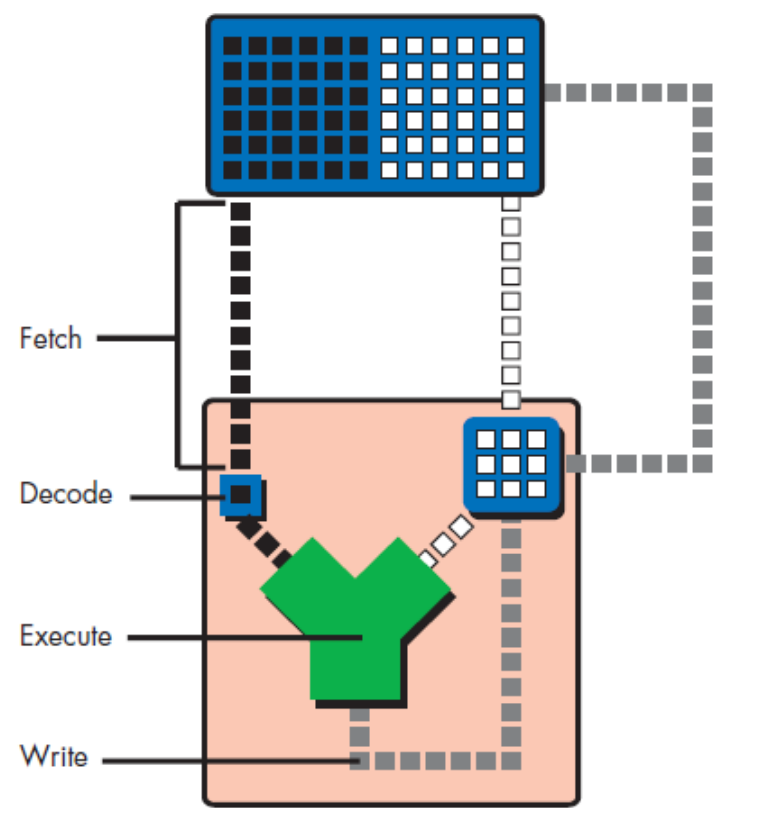
\includegraphics[width=0.65\textwidth]{images/SequenceInstructions.PNG}
\end{center}



\end{document}

